\section{Theoretical Overview}
Path planning in modern video games often involves exploring highly regular 
environments such as cities, sewers or dungeons.
These locales tend to be topographically simple and are frequently comprised only
of empty connected rooms.
It may be somewhat surprising therefore to discover that the canonical A* 
algorithm\cite{hart68} has great difficulties in such domains.
The main problem encountered by A* when traversing across an empty or near-empty 
room is that all generated nodes will have very similar or even identical f-costs.
To preserve optimality A* must expand all such nodes until it can prove they do 
not appear on the optimal path.
Figure \ref{fig-oha_contrast}(a) illustrates such a case; 
notice that A* explores almost half the map. 
\par
To overcome such issues we propose the following simple strategy:
instead of exploring the interior of an empty room expand only nodes along the
perimeter. We claim that this approach preserves optimality when searching in 
4-connected grid maps. 
Consider the following argument:

\begin{theorem}
Every optimal path through the interior of an empty rectangular
room $R$ is dominated by another optimal path involving only nodes on the perimeter of $R$.
\end{theorem}
\emph{Proof} \newline
%\begin{proof}
We refer to Figure \ref{fig-roomtraversal} and let $s$ and $g$ represent
a start and goal location such that $s, g \in R$.
There are two possibilities for exploring $R$: either $g$ is the final goal state
and thus contained in the interior of $R$ or $g$ is an intermediate node on along 
an optimal path which passes through $R$ on the way to a final goal state.
We will show that in both cases there is no need to expand any nodes from the interior of $R$.
\par
First, suppose $g$ is the final goal.
In this case we can simply use a manhattan heuristic to exactly calculate $h*(s, g)$.
Since $R$ is empty the heuristic is perfectly informed and thus equivalent to an optimal
traversal of $R$ but without requring the expansion of any nodes from the interior. 
\par
Next, suppose that $g$ is a node on the perimeter of $R$ and appears on some optimal path to
a final goal node. 
If $g$ is on the same side of the perimeter to $s$ or on one of the two orthogonal sides
it follows we can optimally connect them by simply traversing along the perimeter of $R$.
Suppose however that $g$ is somewhere on the opposide side of $R$. 
In this case we can again use the manhattan heuristic, this time to compute $h*(s, s')$
so that we may generate $s'$; a node in $R$ directly opposite to $s$.
Once $s'$ is generated it follows that $g$ must be reachable from it by simply traversing along
the perimeter of $R$.
\qed
%\end{proof}


 and implies that we can safely prune all nodes from the interior
of an empty 


We posit that on 4-connected grid maps this approach 


solutions in these circumstances.

It is somewhat surprising therefore that the canonical A* algorithm
The canonical A* algorithm has great difficulty in these cases because when
it attempts to traverse an empty room it is 

Overview of our approach.
Notice that in most games related applications large sections
of the map are divided into rooms or other areas. 
Most of the space is empty; we want to avoid expanding all nodes in 
a room unnecessarily.
Give an A* example of CSC2F. 

\begin{figure*}[htbp]
	\vspace{-4pt}
       \begin{center}
                       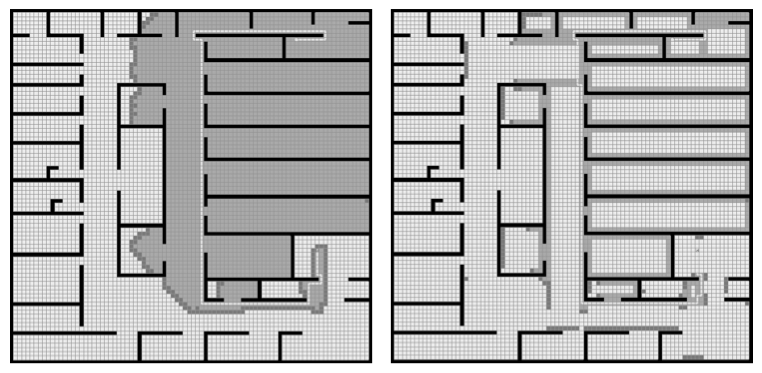
\includegraphics[scale=0.50, trim = 20mm 20mm 20mm 0mm]{diagrams/oha_contrast.png}
       \end{center}
	\vspace{-3pt}
       \caption{\textbf{(a)} An example map and search problem. A* expands all light grey nodes.
			Dark grey nodes denote the frontier of the search. \textbf{(b)} An alternative search strategy involving
			only nodes on the perimeter of empty rooms.}
       \label{fig-ohacontrast}
	\vspace{-12pt}
\end{figure*}

We propose traversing only along the perimeter of these rooms
When the gridmap is only connected in 4 directions such traversals
are optimal because although many paths exist they are all dominated
by a very small number of paths.

Example of our method on CSC2F. 

This approach is optimal because... now give a nice proof.

\subsection{Octile grid maps}.
Explain why this approach doesn't work for 8-connected grids.
